{\LARGE Cybersec threats: ameacas digitais.}
\begin{enumerate}
	\item \href{https://pt.wikipedia.org/wiki/Massacre_de_Columbine}{Tiros em Columbine}
	\item O usuário (sempre ele)
	\item Scammers
	
	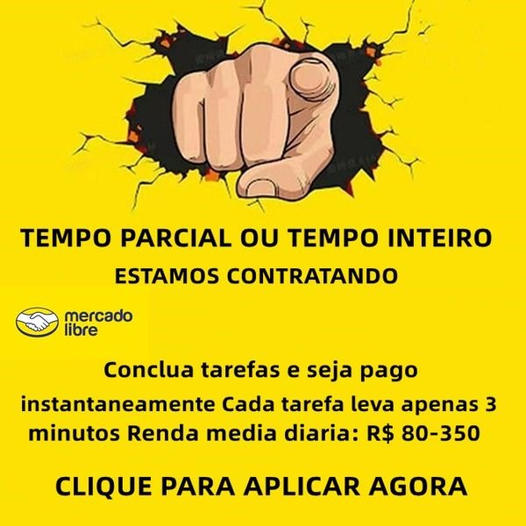
\includegraphics[width=\linewidth]{./IMG/scam.png}
	
	\item Carders
	\item Haters
	\item Trolls: não alimente!
	\item Fake news:
	\begin{enumerate}
		\item Orson Wells e os marcianos.
		\item \href{https://pt.wikipedia.org/wiki/Massacre_de_Columbine}{Tiros em Columbine}
		\item O caso da Escola Base.
		\item A bruxa do Guarujá: o caso Fabiane Maria de Jesus.
		\item A baleia azul.
		\item Nazistas no Brasil.
		\item Ataques às escolas no Brasil.
	\end{enumerate}
	\item Haters: precisamos conversar sobre a Chan.
	\item O tio do zapzap e a tia do Facebook: os haters "bonzinhos".
	\item Mensagens de amor, fé e esperança.
	\item Disparos em massa, para o bem e para o mal.
	\item Ataques de negação de serviço durante o Natal.
	\item Chantagens.
	\item Falso sequestro.
	\item Auto-exposição: suas fotos no Instagram.
	\item Expose: cubra sua webcam!
	\item Expose: não faça besteira!
	\item Manda nudes?
	\item Cancelamento.
	\item Worms.
	\item Trojans.
	\item Virus.
	\item Kiddies.
	\item Engenheiros sociais.
	\item Como Kevin Mitnick foi parar na cadeia.
	\item O caso Boeing.
	\item Lammers.
	\item ILOVEYOU.jpg.
	\item \href{http://g1.globo.com/bom-dia-brasil/noticia/2010/12/menina-de-8-anos-sequestrada-por-prima-escapa-pedindo-ajuda-pelo-celular.html}{Tia, não é um trote. Eu fui sequestrada.}
	\item Minha "namorada"\space no Canadá.
	\item Minha "amiga"\space na Alemanha.
	\item Minha "namorada"\space gaúcha.
	\item Meu amigo na Suíça.
	\item Jogo do Tigrinho: o perigo dos influenciadores digitais.
	\item O coach quântico.
	\item Quando a esmola é demais: golpes diversos.
	
	
\includegraphics[width=\linewidth]{./IMG/DNA-fake.jpg}
	\item Undernet: onde comprar qualquer coisa (qualquer coisa mesmo!).
	\item Servico secretos, inteligência, exércitos e polícias digitais.
	\item A InterPol.
	\item Coleta de dados e vigilância em massa:
	\begin{itemize}
		\item NSA
		\item Google
		\item Facebook
		\item Amazon
		\item Em 200 metros, vire à direita, restaurante a 2 km.
	\end{itemize}
	\item Linux e cyber-segurança nas escolas.
	\item Os hackers de verdade: Estado e Corporações.
\end{enumerate}

\vfill\null
\columnbreak
